\documentclass{article}
\author{
  Torrent Gorjon, Xavier\\
  \texttt{Xavier.TorrentGorjon@os3.nl}
}
\title{Protecting against relay attacks forging increased distance reports}

\usepackage{graphicx}

\usepackage[backend=bibtex]{biblatex}

\bibliography{references}


\begin{document}


\begin{titlepage}
\center
\textsc{}\\[1cm]
\textsc{\LARGE University of Amsterdam}\\[1.5cm]

\textsc{\Large Research Project I proposal}\\[0.5cm]

\textsc{\Huge \textbf Protecting against relay attacks forging increased distance reports}\\[1.5cm]


\includegraphics[scale=1]{images/uva.png}\\[1cm]

\begin{minipage}{0.5 \textwidth}
\begin{center} \large
Xavier Torrent Gorj\'{o}n\\
\emph{Xavier.TorrentGorjon@os3.nl}\\[0.5cm]
\end{center}
\end{minipage}\\[2cm]
{\large \today} 


\end{titlepage}


\newpage

%\tableofcontents
\section{Introduction}
Most communication systems can be secured by using encryption protocols when there is a need to secure user data. This prevents attackers from gaining any information (provided the protocols are correctly implemented and the algorithms have no weaknesses) about the data being transmitted.

However, attackers can still make use of attacks based on relaying information to achieve goals such as system malfunction or even unauthorized access. There are many publications providing practical and real world examples about this problem, such as \cite{francillon2011relay, hancke2005practical, hu2006wormhole}. These publications show that this is a general problem not bound to specific implementations of hardware or software, and depending on the constrains of the used systems (power requirement, size, environment conditions) they can be quite challenging to solve.

There have been many studies providing solutions to these problems, using distance-bonding protocols such as the proposed in \cite{brands1994distance} and \cite{rasmussen2010realization}. These protocols prevent verifying terminals from getting relayed messages reporting legitimate users to be closer than they really are.

However, we couldn't find in the available literature solutions for the opposite problem: malicious users relaying attacks to claim that a legitimate user is further away than he really is. Possible interesting study cases regarding this issue might surveillance drones or automated cars.

Imagine a situation where a squadron of flying drones were used to explore an area. To make sure all the area is being checked, these devices must rely on some kind of protocol to exchange information about their positions so that the whole squadron can reassign positions or change formation as obstacles appear. GPS signals can be used to avoid relay attacks forging distance reports, but it's not a system that we can trust (drones working inside a warehouse, or being on a hostile environment where GPS signals are blocked), so the whole system should be independent from external positioning information. If the drones' system to report relative position to other drones is tempered somehow, it could lead to an attacker successfully preventing an area from being explored or even forcing two or more drones to crash together by making them believe they are further away than they really are.

It is easier to find an exploitable situation on automated car systems, as usually they loose their GPS signals without being in an obviously hostile environment, due \emph{natural} causes such driving inside a tunnel, being on a neighbourhood with tall buildings or stopping at an underground parking.

These study cases are topical issues nowadays, and we find them an interesting subject to work with. They both fall under the category of MANETs (Mobile Ad Hoc Networks) and, treating them as such, the goal of this project will be to provide solutions to the stated problems.

\section{Related Work}

All the papers we found researching on this subject were focused on preventing attacks aimed to fake a closer position, usually related to access systems such as PKES (Passive Keyless Entry and Start Systems) \cite{francillon2011relay} and proximity cards \cite{hancke2005practical}.

Although the proposed solutions for these problems (\cite{brands1994distance, rasmussen2010realization}) are not suitable for our research, they will surely serve as an inspiration.


\section{Research Questions}

In this project we will attempt to answer two main questions:\\

\emph{How feasible it is to perform relay attacks on MANETs which forge reports stating increased distances than the real ones?}\\

\emph{To what extend can we detect, prevent, or provide countermeasures against those attacks?}\\

Answering the first question is a pre-requisite to narrow down the scope of the project and make decisions on how to proceed with the investigation. It is important to study which conditions and attack paths could be available in order to provide a complete picture of the problem.

The second question will be a theoretical research on how can these networks be protected against that kind of relay attacks. It is possible that more than one solution is found, and in that case, a comparison between them will be given, as different solutions will most likely have different advantages and disadvantages over the others.


\section{Planning}

The assigned time for this project are four weeks, from January 5th to January 30th. The presentation and defence of the project will be done on the first week of February. The project development will proceed as follows on the next diagram:

\begin{center}
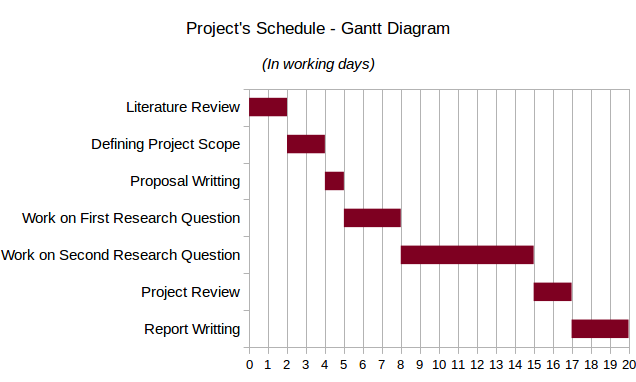
\includegraphics[scale=0.7]{images/gantt.png}\\[1cm]
\end{center}

\section{Expected results}

By the end of this project we expect to provide one or more theoretical solutions and countermeasures to protect MANET from relay attacks on their communication systems that lead to nodes believing they are further apart than what they really are.

\section{Ethical considerations}

The project will be a theoretical study that will not be using any kind of user data, and solutions provide will be based upon theoretical models. We can safely assume that we won't be running on ethical issues regarding user privacy.

At this moment we cannot foresee any direct implications regarding ethical issues, as this project will focus on developing new protocols to protect against a certain type of relay attacks, not on trying to find weaknesses on any theoretical or real application.

\printbibliography

\end{document}
